%-*- ES -*-
%----------------------------------------------------------------------
% Capitulo: Implementacion de la solución propuesta
%----------------------------------------------------------------------

\section{Propuestas: Introducción}

Se han investigado tres alternativas enfocadas en redes internas mara mejorar la seguridad de las 
mismas, luego de eso se eligió la que mas ventajas nos ofreció.
Vimos tres alternativas posibles: Los certificados auto-firmado (Self-signed Certificates), implementar
una entidad certificante interna, y la utilizacion de un certificado emitido por una entidad
certificante conocida

\section{Propuesta 1: Self-signed Certificates}
Los certificados autofirmados son los menos útiles de los tres. Firefox facilita su uso 
de forma segura; crea una excepción en la primera visita, después de lo cual el 
certificado autofirmado se considera válido en las conexiones posteriores. Otros 
navegadores hacen que haga clic en una advertencia de certificado cada vez. A menos 
que esté comprobando la huella digital del certificado cada vez, no es posible hacer 
que ese certificado autofirmado sea seguro. Incluso con Firefox, puede resultar 
difícil utilizar estos certificados de forma segura.

Por ejemplo, para solicitar un certificado SSL de una CA de confianza como Verisign o 
GoDaddy, se debe enviae una Solicitud de firma de certificado (CSR) y te dan un 
certificado a cambio, que firmaron con su certificado raíz y clave privada. Todos 
los navegadores tienen una copia (o acceden a una copia desde el sistema operativo) 
del certificado raíz, por lo que el navegador puede verificar que su certificado 
fue firmado por una CA confiable.

Cuando generamos un certificado autofirmado, generamos nuestro propio certificado 
raíz y clave privada. Debido a que genera un certificado autofirmado, el navegador 
no confía en él. Está autofirmado. No ha sido firmado por una CA. Todos los 
certificados que generamos y firmamos serán de confianza inherente.

La principal dificultad es que los usuarios siempre encontrarán una advertencia 
donde el navegador diga que se encuentra en un sitio con un certificado autofirmado. 
En la mayoría de los casos, no verificarán que el certificado es el correcto, por 
lo que generará desconfianza en los usuarios.

En prácticamente todos los casos, un enfoque mucho mejor es utilizar una CA privada, 
que es nuestra próxima propuesta. Requiere un poco más de trabajo por adelantado, 
pero una vez que la infraestructura está establecida y la clave raíz se distribuye 
de manera segura a todos los usuarios, dichas implementaciones son tan seguras como 
el resto del ecosistema PKI.

\section{Propuesta 2: Internal CA}

(FALTA MAS MARCO TEORICO)
Aca se tiene que decir: "Como se explicó anteriormente, una entidad de certificacion es ..."
Esta alternativa implica establecer una entidad de certificacion interna a la red privada. Esto se hace 
mediente un servidor dedicado que certifique los certificados que circulen internamente.
Como ventaja se tiene que ... 

Ventajas de la autoridad de certificación interna (CA)

• La administración simplificada y fácil es la principal ventaja de utilizar una autoridad de 
certificación (CA) interna. No es necesario depender de una entidad externa para los certificados.

• En un entorno de Microsoft Windows, la Autoridad de certificación (CA) interna se puede 
integrar en Active Directory. Esto simplifica aún más la gestión de la estructura de la CA.

• No hay ningún costo por certificado cuando utiliza una Autoridad de certificación (CA) 
interna.

Desventajas de la autoridad certificadora (CA) interna

• Implementar una autoridad certificadora (CA) interna es más complicado que utilizar una 
autoridad certificadora (CA) externa.

• La seguridad y la responsabilidad de la infraestructura de clave pública (PKI) está 
completamente sobre el hombro de la organización.

• Las partes / usuarios externos normalmente no confiarán en un certificado digital 
firmado por una Autoridad de Certificación (CA) interna.

• La sobrecarga de gestión de certificados de la Autoridad de certificación (CA) interna es 
mayor que la de la Autoridad de certificación (CA) externa.

La desventaja por la que decidí ir por una mejor opcion fue que, se debe establecer 
individualmente en cada uno de los hosts pertenecientes a la red privada que nuestra entidad 
certificante es de confianza, lo que puede llevar a cabo un gran trabajo de los administradores, 
y, aun asi, pueden suceder que en nuestra red se conecten agentes externos a nuestra 
organizacion, por lo que no podremos realizar la configuracion mencionada.

\subsection{Caso de estudio: Creando nuestra Entidad Certificante privada}
\subsubsection*{Servidor DNS con Docker}

Para montar esta propuesta de solución, se debió crear un servidor DNS, que lo que hace
es básicamente mapear direcciones IP a nombres de dominio. Por ejemplo: nuestra página que 
se encuentra en la dirección 192.168.0.202 se pasará a llamar pagina1.salvadorcatalfamo.intra, 
donde salvadorcatalfamo.intra abarca toda nuestra organización y las páginas que se encuentren
dentro de ella. Otra razón por la cual se debe 
crear un servidor DNS, es que los certificados no se pueden otorgar a direcciones IP, por lo 
cual es un requisito obligatorio tener las páginas web direccionadas con nombres de dominio.

Se eligió el servidor DNS CoreDNS ya que es amigable con Docker; sucede que, por cada versión del 
programa, se generan las imágenes de Docker correspondientes. Estas imágenes son públicas y oficiales, 
lo que da confiabilidad y seguridad extra a la hora de utilizarlas. La configuración está formada por 
los siguientes componentes: los archivos de configuración de CoreDNS (corefile) y los sitios que 
nosotros deseemos, en nuestro caso pagina1.salvadorcatalfamo.intra

\noindent El Corefile es el archivo de configuración de CoreDNS. Este define:
\begin{itemize}
    \setlength\itemsep{-0.6em}
    \item Que servidores escuchan en que puertos y que protocolo.
    \item Para qué zona tiene autoridad cada servidor.
    \item Que \emph{plugins} (complementos) se cargan en un servidor.
\end{itemize}

\noindent El formato es el siguiente
\begin{verbatim}
    ZONE: [PORT] {
        [PLUGIN] ...
    }
\end{verbatim}

\noindent ZONE: define la zona de este servidor. El puerto por defecto es el 53, o bien el valor que se le indique 
con el flag -dns.port.

\noindent PLUGIN: define los complementos que queremos cargar. Cada plugin puede tener varias propiedades, por 
lo que también podrían tener argumentos de entrada.

\noindent Nuestro archivo de configuración es el siguiente:
\begin{verbatim}
    .:53 {
        forward . 8.8.8.8 9.9.9.9
        log
    }

    salvadorcatalfamo.intra:53 {
        file /etc/coredns/salvadorcatalfamo
        log
        reload 10s
    }    
\end{verbatim}

A grandes rasgos, lo que indica esta configuración es que va a existir una zona 
“salvadorcatalfamo.intra”, que estará definida por el archivo que se encuentra en 
“/etc/coredns/salvadorcatalfamo”. Por otro lado, el tráfico restante (dominios externos a nuestra red)
será fordwardeado a 
servidores DNS externos (8.8.8.8 y 9.9.9.9). Además se establecieron algunos plugins de logeo y 
de refresco de configuración.

Nuestro archivo “/etc/coredns/salvadorcatalfamo” contiene la siguiente información.
\begin{verbatim}
salvadorcatalfamo.intra.          IN  SOA ns1.salvadorcatalfamo.intra. ...
pagina1.salvadorcatalfamo.intra.  IN  A   192.168.0.124   
\end{verbatim}

Esto en principio es suficiente para nuestro sitio interno, y contiene las direcciones ip de los 
servidores web y entidades certificantes.

Por el lado de Docker, se utilizó un archivo Docker-compose.yml, y un Dockerfile. 
Docker-compose es una herramienta para definir y ejecutar aplicaciones Docker de 
varios contenedores. Compose usa un archivo YAML para configurar los servicios de 
la aplicación. Luego, con un solo comando, se crean e inician todos los servicios 
desde este archivo de configuración. En nuestro caso, se definió de la siguiente 
manera

\begin{verbatim}
version: `3.1'
services:
    coredns:
        build: .
        container_name: coredns
        restart: always
        expose:
            - `53'
            - `53/udp'
        ports:
            - `53:53'
            - `53:53/udp'
        volumes:
            - `./config:/etc/coredns'    
\end{verbatim}

\noindent Por otro lado, el fichero dockerfile está compuesto por las siguientes líneas:
\begin{verbatim}
FROM coredns/coredns:1.7.0
ENTRYPOINT ["/coredns"]
CMD ["-conf", "/etc/coredns/Corefile"]    
\end{verbatim}

En conjunto, establecen la imagen de CoreDNS que se utilizará, los archivos de configuración y
los puertos que se expondrán, entre otras configuraciones.

\subsubsection*{Creación de nuestra CA en Docker}

La estrategia para crear nuestra CA será seguir los pasos que se deberían realizar en un servidor 
habitual, pero partiendo desde una imagen de Docker de Ubuntu (de stock), y luego realizando un 
commit de estas configuraciones. Luego, archivos importantes como el certificado root y la llave
privada deberán resguardarse, o simplemente resguardar el contenedor creado. 

Se utilizó esta estrategia ya que no había imágenes oficiales que nos sirva para tal fin, por el 
simple hecho de que únicamente se requiere tener instalado OpenSSL y tenerlo configurado.

\noindent Como primer paso, corremos una imagen del sistema operativo Ubuntu

\begin{verbatim}
    docker run -it -v $PWD/ca:/root/ca ubuntu
\end{verbatim}

\noindent Dentro del contenedor, ejecutamos los siguientes comandos:
\begin{verbatim}
    apt-get update
    apt-get install ntp
    apt-get install openssl
\end{verbatim}

\noindent Establecer el hostname al contenedor, hay una línea con la ip del contenedor y el nombre del mismo, 
que es utilizado como hostname, en nuestro caso
\begin{verbatim}
    172.17.0.2      080dec560726
\end{verbatim}

\noindent Lo cambiamos por un hostname con el dominio incluido
\begin{verbatim}
    172.17.0.2      ca.salvadorcatalfamo.intra
\end{verbatim}

\noindent Creamos las carpetas para mejor organización
\begin{verbatim}
    mkdir /root/newcerts
    mkdir /root/certs
    mkdir /root/crl
    mkdir /root/private
    mkdir /root/requests
\end{verbatim}

\noindent Creamos un archivo vacío y un archivo que contiene el primer número de serie para los certificados 
\begin{verbatim}
    touch index.txt
    echo '1234' > serial
\end{verbatim}

\noindent Luego hay que crear la llave privada y el certificado root, en este caso nos pedirá una contraseña, si este servidor 
se usará en un ambiente de producción, deberá ser una contraseña compleja.

\begin{verbatim}
    openssl genrsa -aes256 -out private/cakey.pem

\end{verbatim}

\noindent Una vez que generamos la llave privada, la misma será utilizada como entrada en la creación de 
nuestro certificado root. Nos pedirá algunos datos de localización y relacionados a la 
organización

\begin{verbatim}
    openssl req -new -x509 -key /root/ca/private/cakey.pem 
            -out cacert.pem -days 3650
\end{verbatim}

\noindent Cambiamos los permisos de los archivos que creamos
\begin{verbatim}
    chmod 600 -R /root/ca
\end{verbatim}

\noindent Realizamos unas modificaciones en el archivo de configuración, donde indicaremos 
la dirección de los certificados, y algunas opciones de configuración adicionales
\begin{verbatim}
    vim /usr/lib/ssl/openssl.cnf
\end{verbatim}

Una vez que realizamos estos pasos, estamos listos para realizar el commit de la imagen, con esto,
todos los pasos que realizamos (instalar los paquetes, modificar los archivos de configuración, etc)
no son necesarios que se ejecuten nuevamente.

Para realizar un commit, y que nuestro contenedor sea fácilmente identificable, deberemos seguir 
los siguientes pasos

\begin{verbatim}
    docker ps -a        #identificamos el último contenedor utilizado
    docker commit {id_del_contenedor} 
    docker image ls     #Identificamos la imagen recién creada
                        #no tendrá ni repositorio ni tag
    docker image tag {id_de_imagen} ca:1.0  #nombramos nuestra imagen
\end{verbatim}




Ahora cada vez que queramos correr nuestra CA, lo haremos de la siguiente manera:
\begin{verbatim}
    docker run -it -v $PWD/ca:/root/ca ca:1.0
\end{verbatim}

Em el comando anterior, estamos asumiendo que queremos compartir los archivos de la CA con el servidor 
host.

 

\subsubsection*{Nginx con Docker}

Para probar nuestro certificado, utilizaremos una imagen oficial de Nginx, 
los archivos de configuración
son los siguientes:


\begin{verbatim}
docker-compose.yml

web:
  image: nginx
  volumes:
   - ./pagina1:/usr/share/nginx/html:ro
  ports:
   - "80:80"
  environment:
   - NGINX_HOST=pagina1.salvadorcatalfamo.intra
   - NGINX_PORT=80
\end{verbatim}

En el archivo mostrado, le decimos a Docker que utilice la imagen Nginx, 
que nuestros archivos fuentes
van a estar en el directorio \textit{./pagina1} y que exponga el puerto 80, entre otras
 cosas.

\noindent Para ejecutar este contenedor, se debe ejecutar el siguiente comando:

\begin{verbatim}
    docker-compose up -d
\end{verbatim}




\subsubsection*{Creando nuestro certificado}

Para firmar un certificado, tenemos que seguir los pasos mostrados en la figura \ref{figSolCert}
: el servidor donde se alojará la web debe realizar una solicitud, 
luego nuestra CA retornará el certificado firmado. Desde el servidor web en cuestión, se debe 
crear una llave privada:

\begin{verbatim}
    openssl genrsa -aes256 -out pagina1.pem 2048
\end{verbatim}

\noindent Luego, se deberá crear la solicitud de firma de certificado:
\begin{verbatim}
    openssl req -new -key pagina1.pem -out pagina1.csr
\end{verbatim}

\noindent Luego enviamos esta solicitud y la firmamos en nuestra CA, esta solicitud la vamos a colocar 
en el directorio \textit{/root/ca/requests}
\begin{verbatim}
    openssl ca -in pagina1.csr -out pagina1.crt
\end{verbatim}

\subsubsection*{Configuración del certificado en el servidor web}
Una vez que tenemos este certificado, lo colocamos en el servidor web y 
lo configuramos. Para el caso de Nginx, se debe editar el archivo de configuración 
correspondiente a nuestra web, que en este caso es \textit{pagina1.salvadorcatalfamo.intra}
con el fin de que el mismo pueda localizar correctamente los certificados firmados recientemente.
Adicionalmente, se puede obligar a que cada requerimiento sea redirigido a una conexión
segura mediante SSL.

Como se puede ver en la figura \ref{figCAdesc}, aunque el certificado esté configurado, 
el mismo no es confiable ya que nuestra entidad certificante no está importada a nuestro almacén 
local.

\begin{center}
    \begin{figure}   
       \begin{center}
          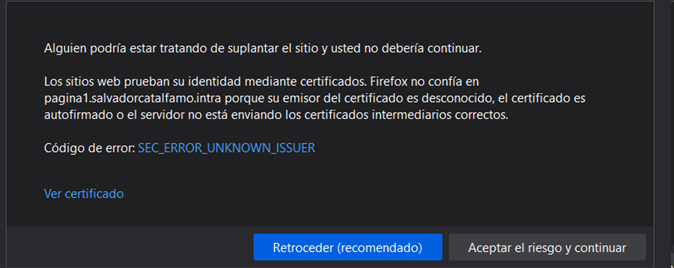
\includegraphics[width=15cm,height=6cm]{adv-2.png}
       \end{center}
       \caption{CA Desconocida}
       \label{figCAdesc}
    \end{figure}
 \end{center}

Luego de establecer en nuestra computadora (particularmente en el navegador Mozilla) que la 
entidad certificante creada es confiable, es posible ver que nuestra conexión es segura, como 
se muestra en la captura.

\begin{center}
    \begin{figure}   
       \begin{center}
          \includegraphics[width=15cm,height=7.5cm]{ca-HTTPS.png}
       \end{center}
       \caption{Resultado de la solución}
    \end{figure}
 \end{center}







\section{Propuesta 3: Cerfification with let's encrypt}
Esta estrategia consiste en generar un certificado wildrau, y utilizarlo en cada sitio de la organizacion
Para esto se debe tener un dominio, en mi caso, salvadorcatalfamo.com, tener la propiedad del dominio
implica poder manejar registros dns del mismo, que es lo que requiere letsencript para poder verificar el mismo
La verificacion es la minima, que es la de que dice cque soy el dueño del dominio
y la verificacion de que cada sitio es mio es la del dns, donde se hace la verificacion con el
registro dns
Entonces, formalmente los requisitos solución
tener el dominio
agregar el registro txt al dns
solicitar la llave publica y privada 
colocarla en cada sitio

\subsection{Pasos a seguir}
\subsubsection*{Get a Domain}
The firs step is getting a Domain, in my case, I had one: salvadorcatalfamo.com.
This domain points to mi public ip address. For that, I had to create some DNS records:


\begin{longtable}{|l|l|p{5cm}|l|l|} 
   \hline
   \textbf{Tipo} & \textbf{Nombre} & \textbf{Contenido} & \textbf{Prioridad} & \textbf{TTL}
\\ \hline A  & salvadorcatalfamo.com & 181.228.121.12 & 0 & 14400
\\ \hline NS  & salvadorcatalfamo.com & ns1.donweb.com & 0 & 14400
\\ \hline SOA & salvadorcatalfamo.com & ns2.donweb.com & 0 & 14400
\\ \hline SOA & salvadorcatalfamo.com & ns3.hostmar.com \newline root.hostmar.com 
                                       \newline 2021010700 28800 7200 
                                       \newline 2000000 86400
                                       \newline ns2.donweb.com & 0 & 14400                  


\\ \hline
\end{longtable}

\subsubsection*{Installing Let’s Encrypt on the server}
\begin{verbatim}
   sudo add-apt-repository ppa:certbot/certbotsudo 
   apt-get update
   sudo apt-get install python-certbot-nginx
\end{verbatim}

\subsubsection*{Installing Nginx}
\begin{verbatim}
sudo apt-get update
sudo apt-get install nginx
\end{verbatim}


\subsubsection*{Obtaining wildcard ssl certificate from Let’s Encrypt}
\begin{verbatim}
sudo certbot --server https://acme-v02.api.letsencrypt.org/directory 
-d *.salvadorcatalfamo.com --manual --preferred-challenges dns-01 certonly
\end{verbatim}

\subsubsection*{Deploy a DNS TXT record provided by Let’s Encrypt certbot after running the above command}
Then I added an entry to my dns records
\begin{longtable}{|l|l|l|l|l|} 
   \hline
   \textbf{Tipo} & \textbf{Nombre} & \textbf{Contenido} & \textbf{Prioridad} & \textbf{TTL}
\\ \hline TXT  & 	\_acme-challenge.salvadorcatalfamo.com & 11UZJD27bPDb\_jFs6f... & 0 & 14400
\\ \hline
\end{longtable}

\subsubsection*{Configuring Nginx to serve wildcard subdomains}

Create a config file sudo touch /etc/nginx/sites-available/example.com

Open the file sudo vi /etc/nginx/sites-available/example.com

Add the following code in the file

\begin{verbatim}
   server {
      listen 80;
      listen [::]:80;
      server_name *.example.com;
      return 301 https://$host$request_uri;
   }
   server {
      listen 443 ssl;
      server_name *.example.com;  ssl_certificate /etc/letsencrypt/live/example.com/fullchain.pem;
      ssl_certificate_key /etc/letsencrypt/live/example.com/privkey.pem;
      include /etc/letsencrypt/options-ssl-nginx.conf;
      ssl_dhparam /etc/letsencrypt/ssl-dhparams.pem;  root /var/www/example.com;
      index index.html;
      location / {
        try_files $uri $uri/ =404;
      }
    } 
\end{verbatim}

The above server block is listening on port 80 and redirects the request to the server block below 
it that is listening on port 443.

\subsubsection*{Test and restart Nginx}
EXTEDER
Test Nginx configuration using 
sudo nginx -t
If it’s success reload Nginx using 
\begin{verbatim}
sudo /etc/init.d/nginx reload
\end{verbatim}
Nginx is now setup to handle wildcard subdomains.

Ver una posible automatizacion, aunque creo que será con puppet

ventajas
No mas mensajes de errores
Seguridad de encriptacion 
privacidad, etc etc

Desventajas
Tal vez la cantidad de dominios gratis
Tal vez la duracion de validez del certificado
Tal vez la confiabilidad

\section{Caso de estudio: Buscando credenciales en tráfico seguro}

Luego de ver las diversas soluciones propuestas, una parte importante de 
nuestro proyecto fue verificar que verdaderamente aumenta la seguridad
cuando nuestro tráfico va encriptado. Para este caso de estudio, se utilizó
el mismo formulario propuesto en la sección \ref{secCaseOfStudy}, lo 
único que con servidores en distintas direcciones.

Dado que el proceso de capturar el tráfico en una red interna fue
explicado previamente, se van a mostrar únicamente los paquetes capturados
desde la primera solicitud hasta el envío del formulario

(IMAGEN)

En esta captura podemos observar que:
\begin{itemize}
   \item No es posible determinar, a diferencia de nuestro caso de 
   estudio, a simple vista cual es el paquete 
   en el cual se envía la información critica.
   \item Viendo el contenido de cada uno de los paquetes mostrados,
   tampoco es posible ver las credenciales completadas en el formulario, 
   que obviamente son de nuestro conocimiento.
   \item Se establece una conexión segura a traves del protocolo TCP.
\end{itemize}


